\documentclass[
reprint,
%preprint,
superscriptaddress,
%groupedaddress,
%unsortedaddress,
%runinaddress,
frontmatterverbose,
%preprint,
%showpacs,preprintnumbers,
%nofootinbib,
%nobibnotes,
%bibnotes,
amsmath,amssymb,
%aps
pra,
%prb,
%rmp,
%prstab,
%prstper,
%floatfix,
]{revtex4-2}

\usepackage{iftex}
\ifPDFTeX
  \usepackage[utf8]{inputenc}
  \usepackage[T1]{fontenc}
\else
  \usepackage[UTF8,scheme=plain,fontset=fandol]{ctex}
\fi

\usepackage{amsfonts,amsmath,amssymb,amsthm}
%\usepackage{ulem}
\usepackage[normalem]{ulem}
\newcounter{fnnumber}
\usepackage{graphicx}% Include figure files
\usepackage{dcolumn}% Align table columns on decimal point
\usepackage{bm}% bold math
%\usepackage{hyperref}% add hypertext capabilities
%\usepackage[mathlines]{lineno}% Enable numbering of text and display math
%\linenumbers\relax % Commence numbering lines

%\usepackage[showframe,%Uncomment any one of the following lines to test
%%scale=0.7, marginratio={1:1, 2:3}, ignoreall,% default settings
%%text={7in,10in},centering,
%%margin=1.5in,
%%total={6.5in,8.75in}, top=1.2in, left=0.9in, includefoot,
%%height=10in,a5paper,hmargin={3cm,0.8in},
%]{geometry}


%%%%%%%%% User specified commands %%%%%%%%%%

\usepackage{hyperref}

\hypersetup{
	pdfborder={0 0 0}
	pdfnewwindow=true,      % links in new window
	colorlinks=true,       % false: boxed links; true: colored links
	linkcolor=blue,          % color of internal links (change box color with linkbordercolor)
	citecolor=blue,        % color of links to bibliography
	filecolor=blue,      % color of file links
	urlcolor=blue,          % color of external links
}

\usepackage{color}
\usepackage{amsmath}
\renewcommand\boldsymbol{\bm}



%%%%%%%%%%%%%%%%%%%%%%%%%%%%%% User specified LaTeX commands.
\usepackage{lineno}
\makeatother
%\usepackage{babel}
%\usepackage{mathabx}
%\usepackage{ulem}
%\usepackage{cancel}

\newcommand{\be}{\begin{equation}}
\newcommand{\ee}{\end{equation}}
\newcommand{\hh}{{\mathcal{H}}}
\newcommand{\bk}{{\bm{k}}}
\newcommand{\br}{{\bm{r}}}
\newcommand{\bR}{{\bm{R}}}
\newcommand{\mR}{{\mathcal{R}}}
\newcommand{\mL}{{\mathcal{L}}}
\newcommand{\mD}{{\mathcal{D}}}
\newcommand{\mG}{{\mathcal{G}}}

\newcommand{\bj}{{\bm{j}}}

\newcommand{\bx}{{\bm{x}}}
\newcommand{\bq}{{\bm{q}}}
\newcommand{\bp}{{\bm{p}}}
\newcommand{\dk}{{d\bm{k}}}
\newcommand{\dr}{{d\bm{r}}}
\newcommand{\ur}{{\bm{u}(\bm{r})}}
\newcommand{\ek}{{\varepsilon_{\bm{k}}}}
\newcommand{\self}{{\mathit{\Sigma}}}
\newcommand{\sn}{{\sqrt{N}}}
\newcommand{\gk}{{\nabla_{\bm{k}}}}
\newcommand{\uk}{{u_{\bm{k}}}}
\newcommand{\ii}{{\mathrm{i}}}
\newcommand{\tr}{{\text{tr}}}
\newcommand{\overbar}[1]{\mkern 1.5mu\overline{\mkern-1.5mu#1\mkern-1.5mu}\mkern 1.5mu}
\def\ket#1{\mathinner{|{#1}\rangle}}
\newcommand{\abo}{{\textit{ab initio}}}


\renewcommand{\thefootnote}{\roman{footnote}}
\newcommand{\bl}[1] {\textcolor{blue}{#1}}
\newcommand{\ma}[1] {\textcolor{magenta}{#1}}
\newcommand{\re}[1] {\textcolor{red}{#1}}
\newcommand{\ZH}[1] {\textcolor{cyan}{[ZH:#1]}}

\newcommand{\LZ}[1]{\textcolor{blue}{[LZ:#1]}}
\newtheorem{thm}{Theorem}
\newtheorem{cor}{Corollary}
\newtheorem{lem}{Lemma}
\newtheorem{dfn}{Definition}
\newtheorem{propdfn}{Proposition/definition}

\usepackage{braket}
\usepackage{array}
\usepackage{booktabs}
\usepackage{multirow}

\usepackage{float}
%\def\thefootnote{$\dagger$}\footnotetext{These authors }\def\thefootnote{\arabic{footnote}}


\newif\ifdraft
\drafttrue
\draftfalse
\usepackage{titlesec}
\titleformat{\section}{\raggedright\bfseries\large}{\arabic{section}.}{1em}{}
\titleformat{\subsection}{\raggedright\bfseries}{\arabic{section}.\arabic{subsection}.}{1em}{}

\titlespacing*{\section}{0pt}{1em}{1pt}
\titlespacing*{\subsection}{0pt}{1em}{0pt}


\begin{document}
\title{标题示例：使用RevTeX4-2撰写科学论文的模板}

\author{Alice Example}
\affiliation{Department of Physics, Example University, Example City 123456, Country}
\affiliation{Example Institute for Advanced Research, Example City 123456, Country}


\author{Bob Researcher}
\email{corresponding.author@example.edu}
\affiliation{Department of Physics, Example University, Example City 123456, Country}
\affiliation{Example Institute for Advanced Research, Example City 123456, Country}

%%%%%%%%%%%%%%%%%%%%%%%%%%%%%%%%%%%%%%%%%%%%%%%%
\begin{abstract}
这里写摘要。这个模板保留了原始导言区中的宏命令和格式设置，并演示中文输入、公式、图片、文献引用与交叉引用的基本写法。
\end{abstract}

\maketitle

\section{Introduction}

这里是正文示例。中文可以直接输入；英文、数学符号和引用可以混排。
例如，这里引用一篇文献~\cite{an_sc1}，也可以同时引用多篇文献~\cite{an_sc1,perdewGeneralized1996}。

交叉引用通常通过 \verb|\label| 和 \verb|\ref| 完成。
例如，式~\eqref{eq:sample-energy} 给出了一个简单的能量表达式，
图~\ref{fig:fig1} 展示了如何插入图片。


图片文件建议放在 \verb|figs/| 目录下。插图示例如下：



\section{Methods}

行内公式可以写成 $E = mc^2$。原始模板中的快捷命令也可以继续使用，
比如 $\bk$、$\br$、$\hh$、$\ket{\psi}$ 和 \abo{}。

独立公式可以写成
\be
  E(\bk) = E_0 + \frac{\hbar^2 |\bk|^2}{2m^\ast}.
  \label{eq:sample-energy}
\ee

多行公式可以使用 \verb|align| 环境：
\begin{align}
  f(x) &= ax^2 + bx + c, \label{eq:quadratic} \\
  \frac{df}{dx} &= 2ax + b.
\end{align}
这里再次引用式~\eqref{eq:quadratic}。

\section{Results}

\begin{figure}[htbp]
  \centering
  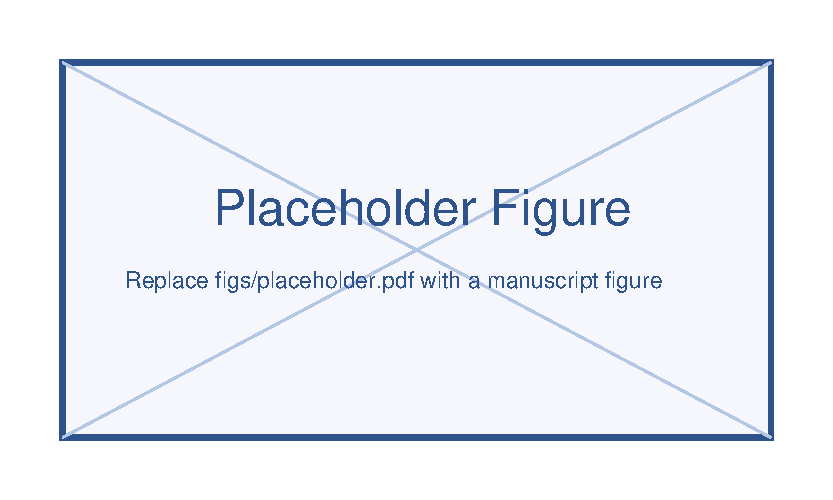
\includegraphics[width= 7cm]{figs/placeholder.pdf}
  \caption{占位图片示例。将实际图片放入 \texttt{figs/} 后，替换这里的文件名即可。}
  \label{fig:fig1}
\end{figure}

\section{Conclusion}

这里写结论。提交前建议运行 \verb|make|，确认文献、公式编号、图片和交叉引用都能正常生成。

\bibliography{ref.bib}

\end{document}
